\chapter{Architecting a Multi-tenant System}
\label{chapter:architecting}
\section{Architecture \& Architecture Description} \index{Architecture Description}
This section briefly introduces concepts covered by ISO/IEC42010. It defines the terms used in the development of the architecture description artefact as well as discusses the architecture modelling language and framework used.


ISO42010 and its predecessor IEEE1471 attempted to establish a coherent practice for developing architecture descriptions, frameworks and architecture description languages \cite{InternationalOrganizationOfStandardization2011}. This in turn required the formalization and standardization of key architecting terms (see table \ref{table:iso_def} on page~\pageref{table:iso_def} for key term definitions). One of the important distinctions made by these standards was between architecture and architecture description (AD). In software architecture refers to the fundamental concepts or properties of a system, in its environment and embodied in its elements, relationships and principles of its design and evolution \cite{InternationalOrganizationOfStandardization2011}. In order to explain this architecture and its components, architects produce a product of work that helps express the architecture as a whole namely an AD. ADs are powerful tools in expressing the core essence of a software system in relation to its key properties, behaviour, composition and evolution \cite{InternationalOrganizationOfStandardization2011}. 

Understanding this essence is also critical in helping us to bring into effect, manage and improve the system in regards to its non-functional requirements. These AD also help address known concerns of stakeholders for a system of interest \cite{Emery2009}. It is therefore an important part of any software or systems life-cycle to produce some form of architectural description to communicate different concerns to the different stakeholders from their respective views throughout. The concerns of the different stakeholders are exemplified through the use of architectural views where each view covers a set of identified concerns and is captured via the use of conceptual or meta-models \cite{42010faq}.


\section{Architecture Description Languages (ADLs)}

An ADL is a set of model, notations and specifications used that are applied in order to describe software architecture and its business domain. For this paper a few ADLs have been considered including the Stanford's Rapide Project \cite{Luckham1996}, WRIGHT ADL \cite{Allen1997} and ACME \cite{bjorn}. Although ADLs are popular amongst scholars and researchers their popularity amongst architects have been questionable outside specialized domains \cite{Woods2005}. In contrast, Unified Modeling Language (UML) has seen widespread adoption by system architects. Although it is not technically considered an ADL, UML provides a set of notations that suffice for creating of general architecture description models \cite{Woods2005}.

\section{UML}

UML was adopted as standard by the Object Management Group (OMG) in 1997. It is the result of a variety of Object-Oriented Analysis and Design methods that were introduced during the 80's and 90's \cite{Fowler2004}. Developed by a team of architects commonly referred to as the "three amigos", UML is a direct result of the work done by Grady Booch, Ivar Jacobson and James Rumbaugh at the Rational software company. After adoption as standard by OMG, UML has received widespread adoption and usage in software and enterprise systems architecture communities. UML2 includes 13 basic diagrams which are generally subdivided into two broad categories for modeling. Firstly, structural diagrams indicate static architectural constructs such as classes, objects and components as well as the relationship between these. Secondly, behavioural diagrams that are used to model the functional or dynamic constructs of an architecture. This thesis uses UML as its ADL.


\section{Architectural Framework}

ISO/IEC/IEEE 42010:2011 (ISO-42010) defines an architecture framework as "a framework establishing a common practice for creating, interpreting, analyzing and using ADs within a particular domain of application or stakeholder community".

\begin{figure}
\centering
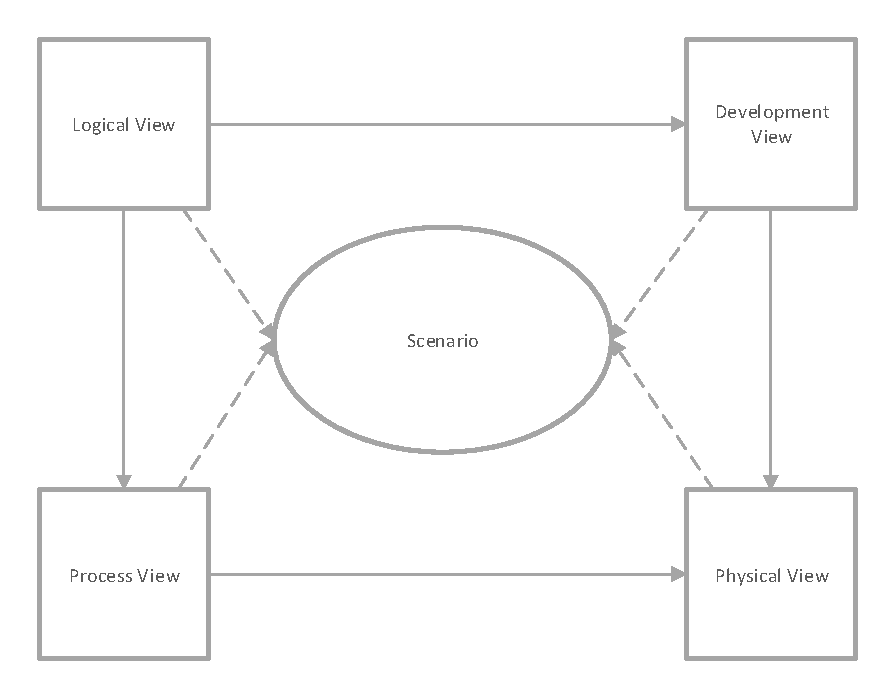
\includegraphics[width=\textwidth]{4plus1frameworksmall}
\caption{4 + 1 Framework}
\label{fig:4plus1frameworksmall}
\end{figure}

The 4+1 Architectural View Model as designed by Kruchten \cite{Kruchten} identified five high level views for use during the creation of an AD (see figure \ref{fig:4plus1frameworksmall}). These views correspond to ISO-42010's view points as they refer to different stakeholder's views and help address these stakeholders' specific considerations. It is important to note that although \cite{Kruchten} uses the term view in his work, ISO-42010 defines the view as the physical work product of an architectural view. A simple breakdown of the 4+1 viewpoints and their mappings to supportive UML diagrams can be seen in Appendix \ref{table:viewpoints} as a composition of \cite{Wiki4plus1}, \cite{Muchandi2007} and \cite{Kruchten}.


This thesis uses the 4+1 framework in order to define the common principles and practices for describing the architecture. This framework is combined with UML in order to provide specific viewpoints from which views are constructed via diagrams of various model types.



\section{Design Concerns in Multi-tenant Systems}
\index{Design Concern}
\index{Multi-tenant}
The architecting of any software or system faces some concerns and challenges; this is also true for multi-tenancy.\index{Multi-tenant} Although many of the challenges encountered during multi-tenant architecting is similar to that encountered in single-tenant application architecting, the challenges are often presented in another form or complexity level for multi-tenant approaches \cite{Bezemer:2010:MSA:1862372.1862393}. This section takes a look at the concerns and challenges faced when architecting a multi-tenant system and attempts to support the ultimately chosen solutions to these.

\subsection{Performance}
\label{sec:performance}
\subsubsection{\textbf{Performance Isolation}}

It is common for single-tenant applications to have one instance consume all available resources. In such a case one tenant's behaviour does not affect another. However, this is not the case for multi-tenant applications where resources are shared and the over-utilization by one tenant does directly impact another. Tenant performance isolation aims to reduce the performance impact between tenants through using fairness policies, throttling techniques or specific design patterns. Since multi-tenant applications aim to be elastically scalable, tenant performance isolation should be designed to support a scaling model and not restrict tenants. This means that assigning of equal amounts of resources between tenants is not an effective solution since it leads to low utilization of resources per tenant \cite{Bezemer:2010:MSA:1862372.1862393}. In order to improve performance isolation in our architecture a Queue Centric Workflow pattern is used (see section \ref{sec:qcw}). 

\subsection{Caching}

In single-tenant applications the use of in memory caching is a quick and easy solution to performance improvement. However, using in memory caching in a multi-tenant environment is not viable, since cached data might need to be shared across multiple application instances. In order to address this, an external cache provider has to be used for maintaining cache data for all application instances. Azure Redis Cache \index{Azure!Azure Redis Cache} is suggested for implementation in the prototype \index{Prototype} as cache provider combined with the the Cache Aside pattern \cite{Homer2014}. Using an external cache instead of in memory caching does introduce some latency as a network component is introduced. As long as the application and its external cache are hosted within the same datacenter however, this latency can be kept to an acceptable minimum.


\subsection{Scalability}
\label{sec:scalability}

\subsubsection{\textbf{Auto-scaling}}

Auto-scaling is the capability of dynamically allocating more or less resources as required by an application on demand and in accordance to some predefined Service Level Agreement (SLA) \cite{Homer2014}. Cloud -Native applications strive to be completely auto-scalable which allows large savings due to the over provisioning of resources. Auto-scalable applications can demand more resources be provisioned when loads are high and could allow resources to be removed when it detects that allocated resources are not being completely utilized. Although implementing a fully auto -scalable application for this thesis would be ideal, as it stands it has been deemed out of scope. However, since it is hard to change a horizontally scalable application to a completely auto-scalable one. Some architectural decisions were made with auto-scaling in mind such as application statelessness and affinity.


\subsubsection{\textbf{Affinity and State}}

In order to improve the performance and scalability of our multi-tenant application, a stateless Web Tier is used. This means that the application requires no affinity, as no specific application instance will store session state data and therefore any instance can handle all application requests. This in effect allows us to scale horizontally without having to worry about maintaining affinity for our users. In cases where some session information has to be stored a client side mechanism is suggested instead. A common client side method is storing specific session data in a cookie using JavaScript Object Notation (JSON). In cases where storing sensitive information on the client side, encryption should be used. When user authentication states are stored in cookies it is also important to remember that attackers that capture the cookie will be able to impersonate that user and therefore protection mechanisms should be put in place e.g. cross site scripting guards.


\subsubsection{\textbf{Multi-Instance Model}}
\label{sec:multiinstance}
\index{Multi-instance}
\index{Multi-tenant}
One major drawback introduced by migrating to a multi-tenant approach is the creation of a single point of failure. That is, that once the instance of the application goes down or is affected by some externality, all tenants are affected and are unable to access the application. If this was to occur, it could be potentially devastating for any service oriented company tied to a SLA. Therefore, some contingency for such a situation is critical to consider, even during the design phase.
 
One possible solution to help mitigate this risk is using a multi-tenant, multi-identical-instance model. That means that the exact same application and roles are replicated to different virtual machines or physical locations. A load balancer is then used to balance the load between these identical instances. In the event that something would happen to one of these instances, the load balancer would then easily be able to switch all requests to the other instance and therefore ensure availability of the application. Azure already provides support for multi-instance models to be deployed and can be implemented using only configuration. Other multi-model supporting features commonly used include Availability sets, Fault Domains and VNets (see section \ref{sec:availability}).


\subsection{Security}
\label{sec:security} 

\subsubsection{\textbf{Dual Input/Tenant Validation (DITV)}}
\label{sec:ditv}
User authentication in a multi-tenant system requires additional security measures. Firstly, users need to be authenticated in order to ensure that they are allowed to access the application. Once a user has been authenticated against the service, they need to be authenticated against the tenant they are claiming to belong to. Only once a tenant has been authenticated to both use the system and access a specific tenant's data is it allowed to be fully authenticated. Furthermore, user requests also need to be checked to ensure they are allowed to be executed against the requested tenant. This forms part of tenant data isolation.


\subsubsection{\textbf{Tenant Data Isolation}}
One of the primary risk factors introduced by multi-tenancy is that of "cross tenant data leakage". An example of this is a case where a CRUD command of one tenant affects or retrieves the information of another tenant. For any application this is behaviour would be unacceptable. It is therefore that proper tenant data isolation is considered one of the essential security factors that needs to be addressed by the systems architect \cite{Wilder2012-so}. By using DITV authentication queries can be analyzed and adapted in order to ensure that they only retrieve information connected to the requested tenant and by an authorized customer.


\subsection{Availability}
\label{sec:availability}
\index{Availability}
In order to control the physical hosting location for your services, Azure requires you to bind your services to a specific region. This region corresponds to the (currently 11) available Azure Data Centres around the world\cite{Microsoft_Corporation2014-bf}. Specifying which region should host your services is equal to selecting the actual data centre where your services will be physically hosted. However, within the data centre it might be beneficial to co-locate services in close physical proximity to each other in order to reduce latency, up performance and cut costs \cite{Microsoft_Corporation2014-dn}.
 

This is where affinity groups come into play. These groups are defined at subscription level and helps Azure to know to group services that belong to a specific affinity group in close physical proximity. Affinity groups are tied to regions.
 
It is important to note that with recent changes in Azure Virtual Network structures that the VNets are no longer tied to affinity groups, but directly associated with the regions. This means that when you create your VNet and affinity group, they should both be located in the same region \cite{Microsoft_Corporation2014-dn}.

\subsection{Configuration and Customization}
\label{sec:custandconf}

The degree to which individual customers are able to customize anything from layouts to schemas should be carefully considered during the application design stages in order to ensure that the architecture allows for sufficient customization from the start. Krebs states that the ability to handle different tenant specific configurations regarding the User Interface (UI) as well as other functional or non -functional behaviour is can be considered as key enabler for multi-tenant applications \cite{Krebs2012}. Since tenants will require some changes or modifications such as extended features, implementation of these features should not influence other parts of the system.
 
The customization required by our multi-tenant application proves to be one of the core elements driving many of the design choices. Each tenant requires complete customization of the front-end to fit their respective Corporate Identity (CI) as well as lower level extension to the system such as publisher filtering on database level. This essentially means specific publishers should only be shown to specific tenants, and some to all. Other important customization considerations include workflow processes used by different clients and how workflows would be implemented to include possible changes by the client.


\subsubsection{\textbf{Tenant Customization}}
\label{sec:viewengine}
In many multi-tenant systems the difference between tenants is minor and can usually be handled by storing the differences in configuration. Settings such as Corporate Identity (CI) which includes fonts, colours and logos or even which parts of the service that has been enabled or disabled is retrieved from the external configuration and applied. However, in our system, this level of configuration is not enough. The XVA requires high levels of modification for the front-end for each tenant. Although the development of highly configurable software is not commonly the responsibility of the multi-tenant application \cite{Krebs2012}, the specific of implementing such an application has been considered during the architecture design. As such, custom views are a robust solution for implementing tenant specific customizations. Custom views effectively allow us to create different views for each tenant, customizing the HTML and CSS for that view to the tenant's requirements. It also allows us to create a custom master or layout view that can be used to apply the tenants CI. This solution could also allow us to use shared views for situations where tenant specific customization is not required. In order for our custom view solution to be applied in ASP.NET \index{ASP.NET} MVC,\index{Model View Controller (MVC)} we create a custom view engine. View engines are primarily responsible for rendering the code from your views into HTML that is served by the browser.

However, View Engines are also capable of defining search paths and retrieving specific views to be served. It is these capabilities that are used to allow our application to search for, and retrieve tenant specific views. Since our requirement does not include any customization to the way views are rendered, extending an existing view engine such as Razor is the most viable option. Morris \cite{Morris} provides a good example implementation of such an extended Razor view engine that allows for multi-tenancy. His approach is implemented in the prototype. A major drawback of using custom views is it removes our ability to dynamically provision new customized tenants. If the tenant's configuration is stored separately from the system following the external configuration store pattern, \cite{Homer2014} new tenants can be provisioned dynamically without any modified views. However, since adding views to a project requires the project to be rebuilt, a new deployment will have to be made when custom views are added. For our case however the high customizability provided by custom views outweighs the drawback of having to constantly redeploy. In order to ease the influence of constant redeployments, using of a continuous integration workflow is strongly suggested.


\subsection{Maintenance}
\label{sec:maintainance}
Bezemer \& Zaidman \cite{Bezemer:2010:MSA:1862372.1862393} state that using multi-tenancy could result in a maintenance dream since application deployment is significantly simplified. By using a single instance of the application and database, any changes simply need to be deployed once. However, this simplified maintenance is closely coupled with implementation quality. High quality multi-tenant application utilize a layered architecture that has multi-tenancy applied as a cross cutting concern \cite{Bezemer:2010:MSA:1862372.1862393}.


\subsubsection{\textbf{Provisioning}}

Since adding tenant specific views requires redeployment, provisioning of new tenants with their custom views in our system will not be an automated process. Tenants can, however, be created dynamically as tenant data is stored externally. This means new tenants can be provisioned without a redeploy, but will only have the generic shared or default views set. In order to properly provision a new custom tenant however, the tenant's specific views can firstly be created, a deployment done and once the tenant needs to be activated it can be created dynamically by an application manager. Once the tenants data has been stored, the application will then be able to automatically associate the custom views with that tenant and start serving the tenant specific customized views. This provisioning process works for our specific case study since a new tenant is usually slowly introduced and requires such high levels of view customization. Multi-tenant systems that have large numbers of tenants (10+) should however rather consider moving away from custom views into a more generic configuration based customization approach, especially where tenant provisioning should be completely dynamic and automated. One method helping to reduce the impact of redeployment for tenant provisioning is by using a build server such as TeamCity combined with a continuous deployment, integration and delivery strategy.


\subsection{Persistence Design}

In multi-tenant system design many different approaches to designing a persistence model can be taken including \cite{Krebs2012}:

\begin{itemize}
\item Dedicated database: Each tenant has their own specific database. This approach offers the highest level of tenant isolation but is considered the least effective multi-tenant approach since it does not attempt to share resources. Allows the high levels of schema customization per tenant.
\item Dedicated table/schema: Tenants share a single database but have their own dedicated tables within that database. This approach is considered better at resource sharing but still does not allow high enough levels of resource sharing. Cross tenant queries for reporting purposes are also harder to implement with this approach. Furthermore, this approach allows high degrees of schema customization.
\item Shared table/schema: All tenants share a single schema or table and provide means for schema extension through extension columns. This approach is considered the purest multi-tenant approach but implores restrictions on schema modification.
\end{itemize}


Since our application requires a constantly varying schema, using a schema-less database has been chosen. This allows us to obtain the highest degree of flexibility. In order to allow the most effective persistence design to be implemented, a shared database, dedicated collection approach was taken. This approach is similar to the dedicated table/schema approach in the sense that a single database is used by all tenants but each tenant has their own respective collection (groupings of documents, searchable indexes, entities etc.). Furthermore since a single data storage type does not fit all our specific needs, such as auto-indexing of fields for searchable items and easy persistence of JSON objects as query-able documents, a polyglot persistence\index{Polyglot persistence} model is used.


\subsubsection{\textbf{Polyglot Persistence Model}}

The term polyglot persistence is used to refer to the utilization of different data stores and types in order to store data \cite{Sadalage2012-zw}. This means that systems information is stored in various different databases with different schemas and models in order to be used for their intended purpose and by providing the required benefits for that specific data storage type. For this thesis a polyglot persistence approach is taken by storing specific data into different databases and different database types. Media items that should be searchable, quickly queried and should have powerful search and filtering features such as geosearch are stored in Azure Search \index{Azure!Azure Search} (Database). This allows all media items to use an easily modifiable schema (at code level), while providing full text search and fully indexed objects for quick and constant queries. The marketplace data is stored in Azure Document DB \index{Azure!Azure Document DB} since the document storage is fast and easy to use. It allows more complex querying compared to key-value store typed storage and allows us to persist objects directly into the database without the need to use an ORM mapper. Finally for identity information, traditional Azure SQL is used since these work well with existing identity providers and have been optimized to work out of the box such as Open Web Interface for.NET (OWIN). Stateful data such as a user's shopping cart or selected media items is stored using Azure Cache and client side cookies. This specific separation of persistence allows us to gain the benefits of each of the respective persistence technologies at the cost of introducing higher code complexity.


\subsection{Accessibility}

One of the most common ways to distinguish between tenants is using the tenant's name as area and mapping the tenant name as an area using MVC routing. However XV tenants wish to maintain their own Domain Name System (DNS) names and access to the system should therefore be setup using sub domains. A suggested method for doing this is setting up a Canonical Name Record (CNAME) entry with our DNS provider that points all domains via the "*" wildcard to the application instance. This will allow us to have tenants to set up their DNS to point to <tenant-name>.<our-domain>.


\section{Conclusion}
This chapter took a look into the Architecture Description standard for Systems and software engineering outlined by ISO4210. It also introduced the Architecture Framework used to present our description namely the 4+1 View Model. Finally it discusses a combination of common high level design concerns encountered in multi-tenant and cloud applications and possible ways of addressing them. 